 \documentclass[12pt]{article}
\usepackage{url,graphicx,tabularx,array,geometry,amsmath,tikz}
\usepackage{algorithm}% http://ctan.org/pkg/algorithms
\usepackage{algpseudocode}% http://ctan.org/pkg/algorithmicx
\usetikzlibrary{arrows}
\setlength{\parskip}{1ex} %--skip lines between paragraphs
\setlength{\parindent}{0pt} %--don't indent paragraphs
\newenvironment{myindentpar}[1]% %indent whole paragraph when needed
 {\begin{list}{}%
         {\setlength{\leftmargin}{#1}}%
         \item[]%
 }
 {\end{list}}
%-- Commands for header
\renewcommand{\title}[1]{\textbf{#1}\\}
\renewcommand{\line}{\begin{tabularx}{\textwidth}{X>{\raggedleft}X}\hline\\\end{tabularx}\\[-0.5cm]}
\newcommand{\leftright}[2]{\begin{tabularx}{\textwidth}{X>{\raggedleft}X}#1%
& #2\\\end{tabularx}\\[-0.5cm]}
%\linespread{2} %-- Uncomment for Double Space
\begin{document}

\title{ECS 256 - Problem set 1}
\line
Olga Prilepova, Christopher Patton, Alexander Rumbaugh, John Chen, Thomas Provan


For this assignment, we adopt the following notation. Suppose $W$ is a random
variable exponentially distrubted with mean $\mu$. Then 
$W \sim \mathcal{E}(\frac{1}{\mu})$.

\subsection*{Problem 1}

\textbf{(a)} $w = 0 \cdot \pi_0 + 1 \cdot \pi_1 + 2 \cdot \pi_2 = \pi_1 + 2 \pi_2$. 

\textbf{(b)} Program is \texttt{1B.R}.

\textbf{(c)} Program is \texttt{1C.R}.
\begin{figure}[h]
  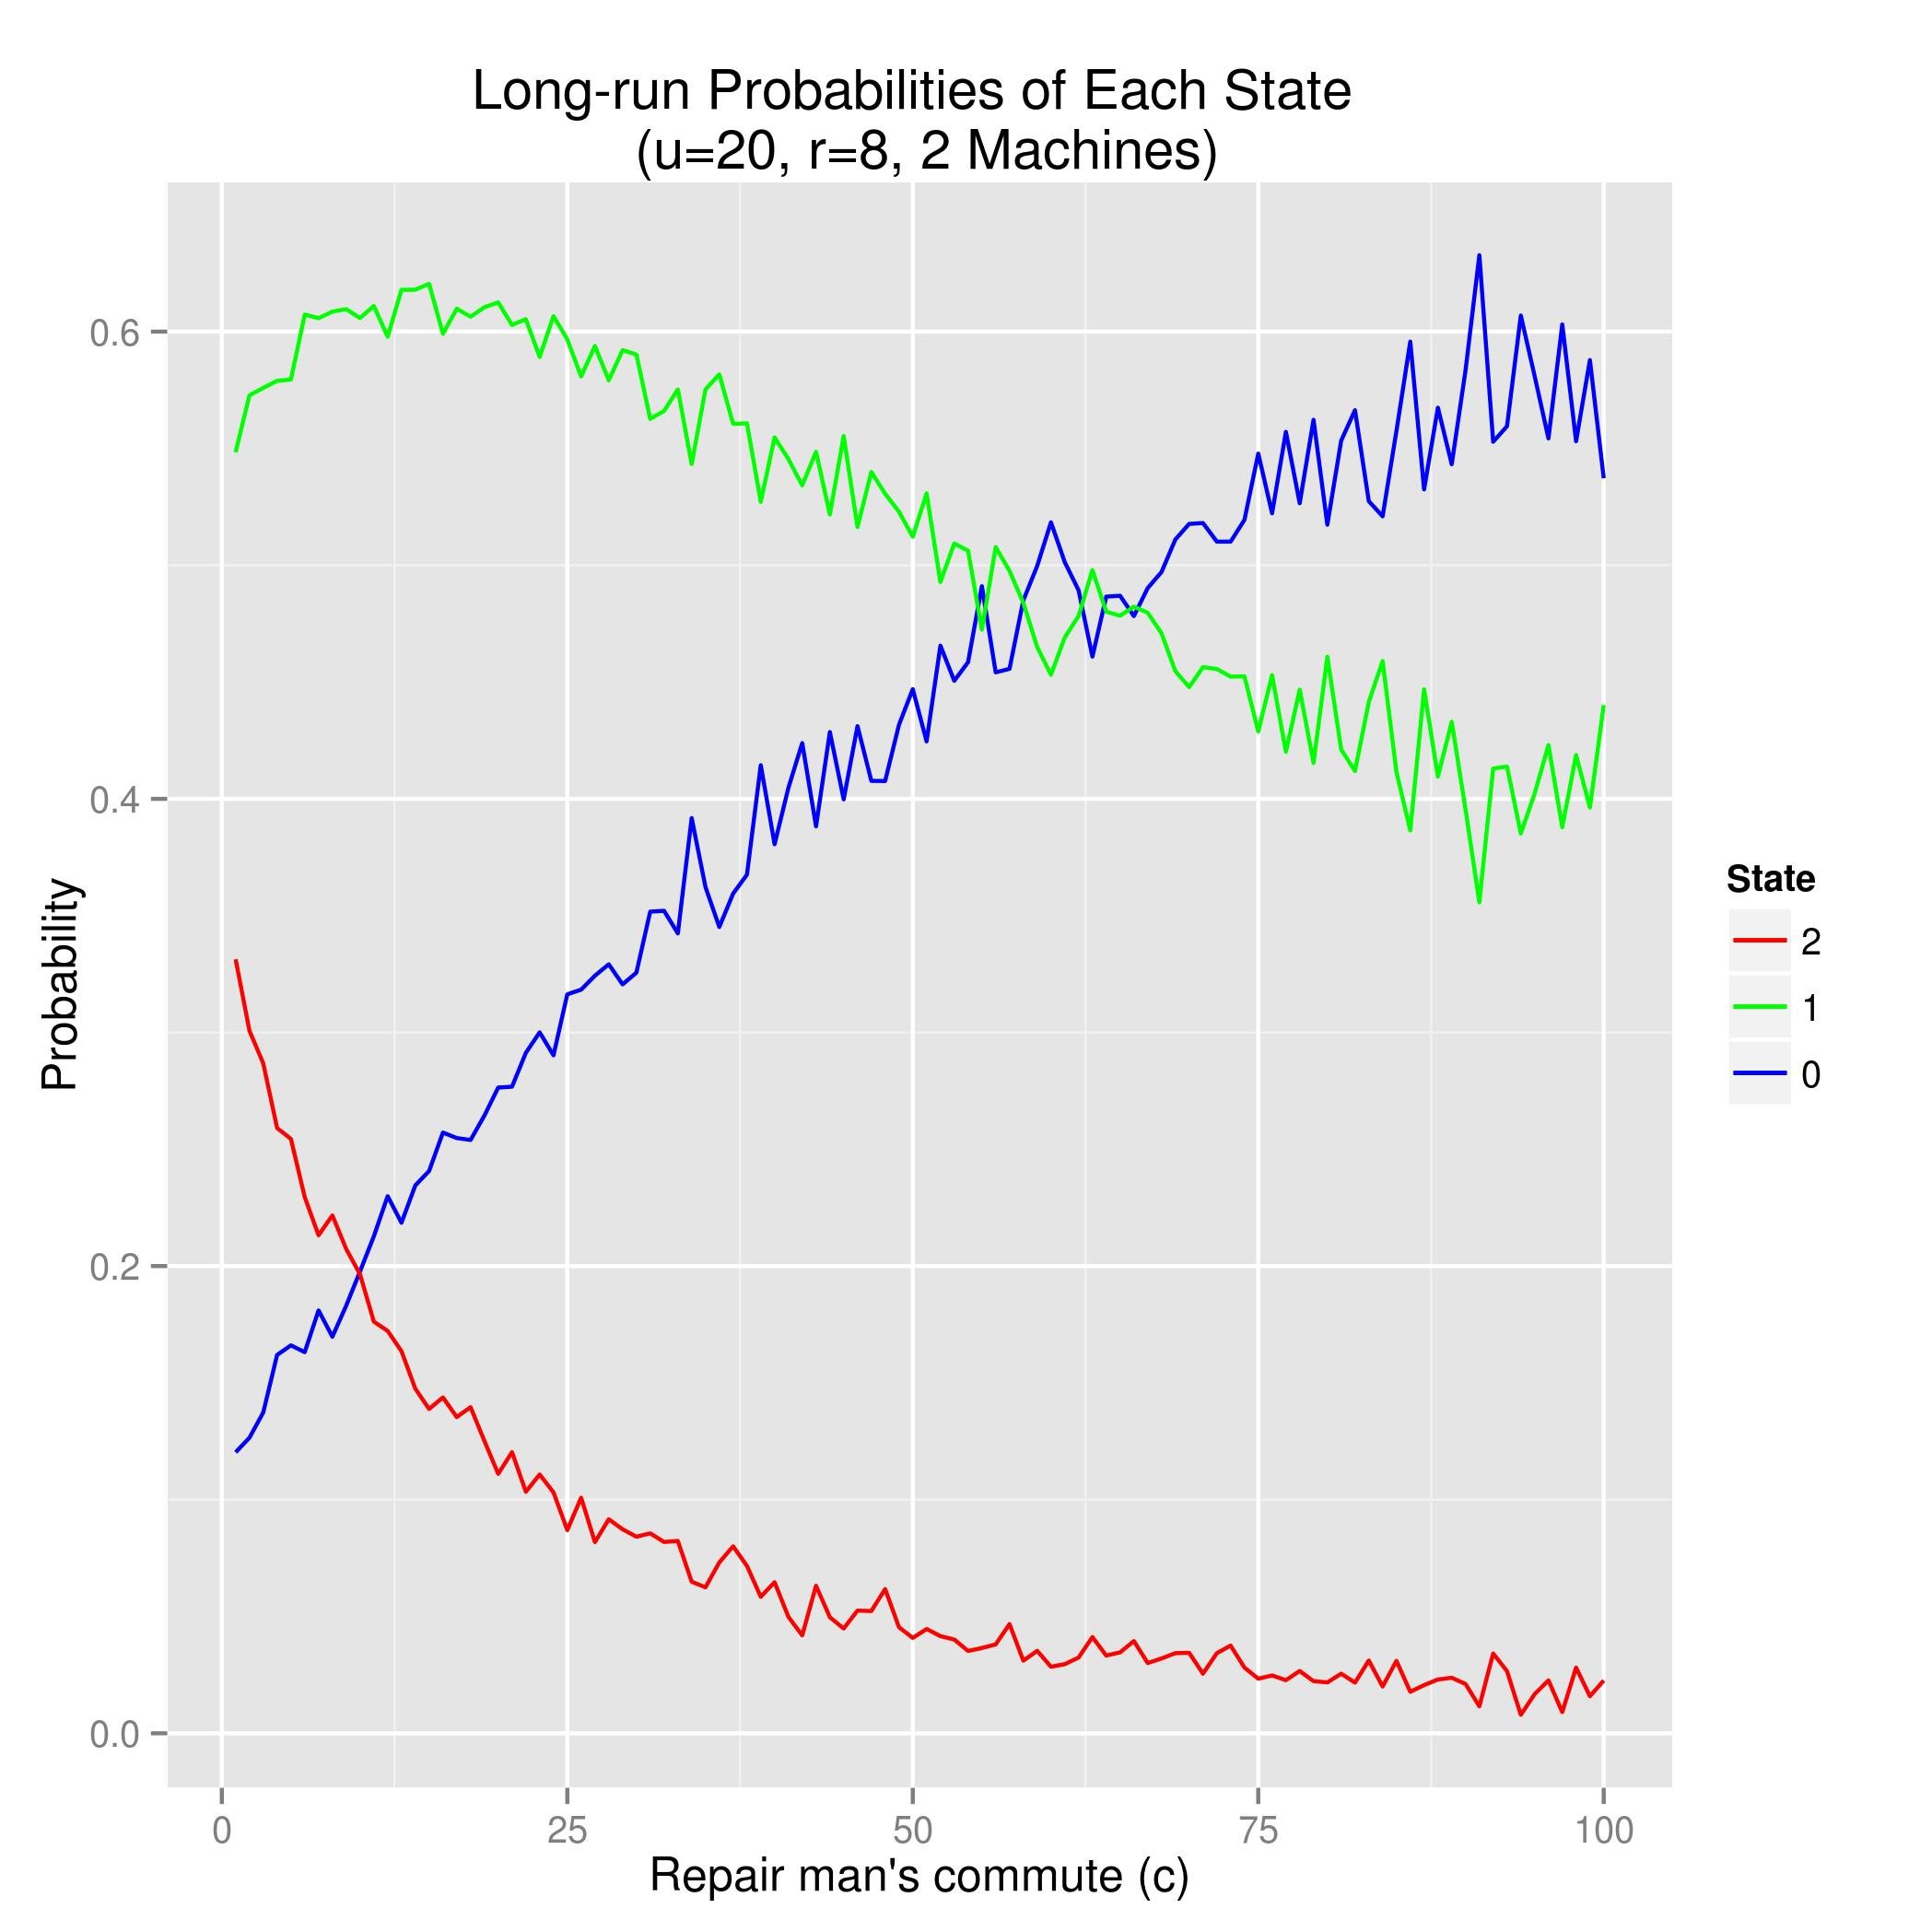
\includegraphics[scale=0.7]{1C.jpg}
\end{figure}
\pagebreak


\subsection*{Problem 2}

\textbf{(a)} Let $D \sim \mathcal{E}(1/d)$ be a random variable corresponding 
to the call druation and $R \sim \mathcal{E}(1/r)$ the time between queued calls. 
The balance equations for the call system: 
$$ \pi_{(i,j)}\lambda_{(i,j)} = \pi_{(i,j-1)}\lambda_{(i,j-1)}p_{(i,j-1)(i,j)} + 
                                \pi_{(i,j+1)}\lambda_{(i,j+1)}p_{(i,j+1)(i,j)} 
  \quad (\forall \quad 0 < j < q, 0 < i < n)$$

$$ \pi_{(i,0)}\lambda_{(i,0)} = \pi_{(i+1,0)}\lambda_{(i+1,0)}p_{(i+1,0)(i,0)} + 
                                \pi_{(i,1)}\lambda_{(i,1)}p_{(i,1)(i,0)}
  \quad (\forall \quad i < n)$$
$$ \pi_{(i,q)}\lambda_{(i,q)} = \pi_{(i,q-1)}\lambda_{(i,q-1)}p_{(i,q-1)(i,q)}
  \quad (\forall \quad i > 1)$$
$$ \pi_{(1,q-1)}\lambda_{(i,q-1)} = \pi_{(i-1,q)}\lambda_{(i-1,q)}p_{(i-1,q)(i,q-1)} 
  \quad (\forall \quad i > 1)$$

$$ \pi_{(n,0)}\lambda_{(n,0)} = \pi_{(n,1)}\lambda_{(n,1)}p_{(n,1)(n,0)} $$ 
$$ \pi_{(1,q)}\lambda_{(1,q)} = \pi_{(1,q-1)}\lambda_{(1,q-1)}p_{(1,q-1)(1,q)} $$

$$ \pi_{(1,0)} + \dots + \pi_{(1,q)} + \dots + \pi_{(n,0)} + ... + \pi_{(n,q)} = 1 $$

\textit{Proportion of rejected calls.} The long-run probability that the call center
is in a state in which it's rejecting calls is the following quantity: 
$$ \sum_{i=1}^n{\pi_{(i,q)}}$$

\textit{Proportion of nurse idle time.} \textbf{TODO}

\textit{Mean time spent in state $(1,1)$.} The possible transitions from this state are 
$(1,0)$ (nurse finishes call, takes next on queue) and $(1,2)$ (call comes in 
before nurse finishes with current call). The time spent in this state is then 
$Z_{(1,1)} = \min \{ D, R \}$. By theorem, $Z_{(1,1)} \sim \mathcal{E}(1/d + 1/r)$. Thus,
the mean time spent in this state is: $$ \frac{1}{\frac{1}{d} + \frac{1}{r}} $$ 

\textit{Given the queue is emtpy, long-run probability that $A_t$ is greater than 1.} 
The sum of the stationary probabilities where $j=0$ and $i>1$: 
$$ \sum_{i=2}^n{\pi_{(i,0)}} $$



\end{document}
